\section{Introduction}
Mobile devices today run many third party applications to perform complex tasks like web browsing, banking and gaming. Recent studies have found that smartphones are the target of an increasing number of malware attacks \cite{bose2006mobile},  \cite{cybercriminals2007banks},  \cite{iphone2010seriot} and their security is important as personal data such as contacts, credit card numbers and passwords are often stored on the device. While some security models \cite{androidsecurity} provide a stronger process level isolation among applications, operating system bugs such as \cite{kernel2009vulnerability}, \cite{opencore2009android}, \cite{sms2009iphone} allow malicious applications to take over the device. We believe that virtualization can be useful for secure isolation of third party code from confidential data and provide a greater defence-in-depth against attacks on the system.\\

In recent years, virtual machines have become prevalent in cluster computing environments \cite{gartner2009virtual} as they lower power costs and help in conserving data center space. Hardware improvements have meant that smart phone configurations found today resemble desktop machines from few years ago and many of them run commodity operating systems. There is a growing interest in academia \cite{cox2007pocket} and industry \cite{vmware2009nextfrontier} about the benefits of virtualization on these devices. We believe that virtualization can provide better security guarantees in mobile devices and enable useful applications like environment migration. \\

Environment migration has been studied earlier, in the context of servers in a cluster \cite{clark2005live} and enables administrators of clusters to perform maintainence tasks without interruption. On the other hand, migrating a system to a mobile device can take advantage of network or computation facilities that are closer to the user's location and provide the user with a consistent experience irrespective of the network connectivity. Migration techniques also help maintain consistent snapshots which allow easy transfer of data when users switch mobile phones and to roll-back the system to a previously known state.

{\bf NOTE: Need to mention OK-L4 and  ARM Trustzone \newline}
\subsection{Existing Work}
Currently, there are many solutions available for virtualization on desktop environments.  VMware is a popular closed source solution which implements a variety of virtualization techniques and is used in both industry and academia.  KVM \cite{kvm}, QEMU \cite{qemu}, and XEN \cite{xen} are all open source solutions, implementing their own assortments of virtualization techniques.  These solutions for the most part do not work well in a mobile environment for performance, security, and usability reasons. \\

Recently there has been a surge of research done for mobile virtualization.  One such solution is MobiVMM \cite{mobivmm}, which prioritizes performance and security at the cost of usability and portability.  Work has been done to port KVM to Android \cite{columbia}, focusing on performance and functionality.  All of these solutions either dual-boot the OS or require disabling the phone's existing runtime stack to use them. \\

VMware's MVP project \cite{mvp} is most similar to ours.  They introduce a very thin hypervisor with an emphasis on usability, performance, and security--without sacrificing the phone's functionality.   However their implementation does not integrate with the host OS, but rather replaces and contains it.  This is useful, but tangential to our work.  As described in Section \ref{oursbetter}, we aim to provide a Type II VM and prioritize live migration capabilities as well as usability.  Furthermore, we are mostly concerned about containing applications for isolation, security, usability, and portability.  Instead of virtualization the existing OS to protect others from it, we assume it is trusted and only have to isolate new applications.  This provides for a very different architecture in our implementation. \\
%We use an idea similar to their JeOS to provide a minimal guest OS when virtualizing appliances.

\begin{figure}[tbh]
\centering
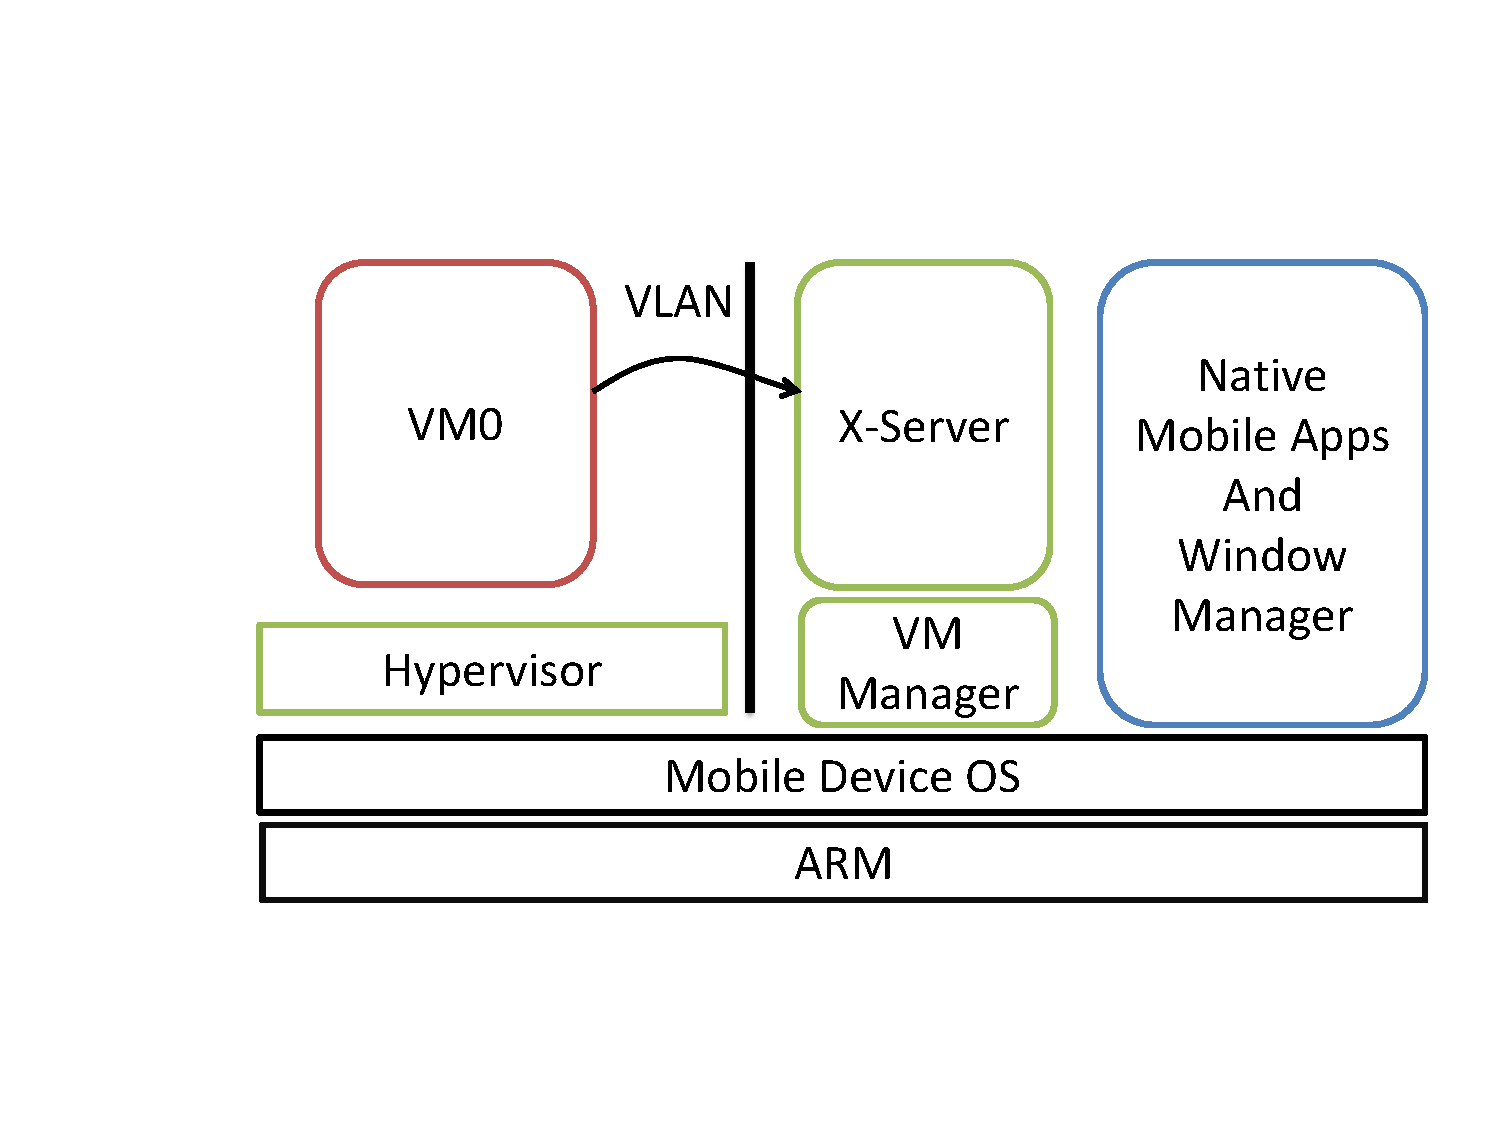
\includegraphics[width=1.0\columnwidth]{arch}
\caption{Architecture diagram}
\label{fig:arch}
\end{figure}

{\bf NOTE: Add some discussion about power usage, memory constraints ? \newline}
%% This subsection really needs a better title!
\subsection{Our solution}
\label{oursbetter}
% this section sucks, feel free to completely rewrite it, or I will at some point.
%XXX: Perhaps we should merge this with the above subsection, and let the 'proposed architecture' section describe what we're doing--and not have to worry about constantly pointing out how what it does is different than ever other mobile virtualization solution
We intend to improve upon the existing mobile virtualization solutions through superior usability.  By integrating with the host OS and building upon the existing user experience and bring added value to existing devices.
A primary goal of ours is compatibility with existing x86 and x11 applications such that upon our project completion we can immediately take advantage of the vast quantity of applications that already use these.
We also provide emulation which appears to the user to be at the application level, making it simpler conceptually to work with.
Our biggest contribution is the way we bring live migration into this.  This is the most novel part of our program.

\subsection{Proposed Architecture}
\label{proposedarch}
%Here describe what we propose to do, perhaps?
%Our timeline/evaluation are kinda worthless without it.
In order to retain the Android application functionality, we plan to virtualize our x86 apps in addition to running the Android runtime stack.  The x86 vms will be run on top of QEMU with Android as the host OS.  X11 will be ported to Android and integrated to run cleanly with the current window manager as well as the vms.  
